
\documentclass[a4paper,10pt]{report}
\usepackage[utf8]{inputenc}
\usepackage{graphicx}
\usepackage[utf8]{inputenc}

%opening
\title{Cahier des charges}
\author{Isabelle Richard, Elias Abou Haydar, Mikael Ahl et Jeremie Rouach}

\begin{document}
\maketitle

\section{Introduction}
\subsection{Objectif du document de specification} 
Ce document de spécification produit des informations spécifiques et\\
nécessaires pour définir efficacement les fonctionnalités, l'architecture et la
conception du système afin de donner la direction à l'équipe de développement
sur l'architecture du système à développer. Le document de spécification du
produit
est créé pendant la phase de planification du projet. Son public visé est le
chef de projet, l'équipe de projet et l'équipe de développement et en partie le
client. Les spécifications techniques et fonctionnelles de ce document sont
réservées au chef de projet, l'équipe de projet et l'équipe de développement.

\subsection{Portée du produit}
Le logiciel iFind permet de rechercher un fichier dans un ensemble de
répertoires ciblés du système. Cette recherche peut se faire soit en indiquant
le nom du fichier, soit en donnant une liste de mots contenus dans ce fichier.

\subsection{Définitions, acronymes et abréviations}
\begin{description}
\item[UI]
Acronyme de “user interface” (interface utilisateur).

\item[Corpus]
Un corpus est un ensemble de documents, artistiques ou non ( textes, images,
vidéos, etc. ) , regroupés dans une optique précise. 

\item[Fichier ]
 Contenant virtuel auquel est assigné un nom unique, permettant de classifier et
de réunir en une même entité une séquence de données. Le fichier est stocké dans
un système de fichier et les données qu'il contient sont généralement
structurées en suivant un même format.

\item[Document]
En informatique, le mot \textit{document} est généralement synonyme de fichier.
On
parle ici de document électronique. Un document électronique est un contenu de
médias électroniques ( autres que les programmes d'ordin\\-ateur ou des fichiers
système ) qui sont destinés à être utilisés soit dans une forme électronique ou
comme sortie imprimée.

\item[Indexation]
L'indexation permet de regrouper en un seul endroit toutes les données
souhaitées. On crée des indexes, ce qui permet d'y accéder plus rapidement. 

\item[Index]
Un index est, en toute généralité, une liste de descripteurs à chacun desquels
est associée une liste des documents et/ou parties de documents auxquels ce
descripteur renvoie. Lors de la recherche d'information d'un usager, le système
accèdera à l'index pour établir une liste de réponses. 

\item[Moteur de recherche]
Un moteur de recherche est un code logiciel qui est conçu pour rechercher des
informations ou retrouver des ressources associées à des mots quelconques. Ici,
on parle de moteur de recherche de type “ Desktop ” , car son champ d'action est
limité à l'ordinateur sur lequel l'application est installée. 

\item[Requête]
 En informatique, une requête est une demande de traitement. Dans notre cas, le
terme est employé dans le contexte des bases de données, une requête
correspondant à l'interrogation d'une base pour en récupérer une certaine partie
des données.
 
\item[Base de données]
 Une base de données, usuellement abrégée en BD ou BDD, est un ensemble
structuré et organisé, permettant le stockage de grandes quantités de
d'informations afin d'en faciliter l'exploration ( ajout, mise à jour, recherche
de données ). Autrement dit, il s’agit d’un conteneur informatique permettant de
stocker dans un même endroit l'intégralité des informations en rapport avec une
activité. Une base de données permet de stocker un ensemble d'informations de
plusieurs natures ainsi que les liens qu'il existe entre les différentes
natures.

\item[Expression régulière]
 Les expressions régulières ( aussi appellées expressions rationnelles ) sont de
chaines de caractères permettant de décrire un ensemble de variables par
l'utilisation d'une syntaxe précise qui se retrouvent dans de nombreux langages
et outils.
 
\item[Démon]
 Un démon ou daemon désigne un type de programme informatique, un processus ou
un ensemble de processus qui s'exécute en arrière-plan plutôt que sous le
contrôle direct d'un utilisateur.
\end{description}

\subsection{References}
IEEE Std 830-1998 Recommended Practice for Software Requirements Specifications 



\section{General Overview and Design Guidelines}
Cette section décrit les principes et les stratégies qui seront utilisées comme
des lignes directrices lors de la conception et de la mise en œuvre du système.

\subsection{Perspective du produit}
iFind utilise une base de données construite à l'aide d'un moteur d'indexation
et mise à jour dès qu'un fichier est modifié. 
La requête est envoyée au moteur de recherche via une interface graphique (GUI)
(voir Figure 1). 
On utilise une interface graphique, pour permettre à l’utilisateur de rechercher
ce dont il a besoin.
La GUI est constituée d’un champ de saisie, d’un bouton “Chercher” ainsi que
d’un explorateur qui permettra d’ouvrir les fichiers trouvés (extension). 
De base, l’explorateur contiendra un tableau dans lequel on affichera les
résultats. 
Le champ de saisie reçoit une requête sous forme d’expression régulière ou des
mots simples. 

\begin{figure}
<<<<<<< HEAD
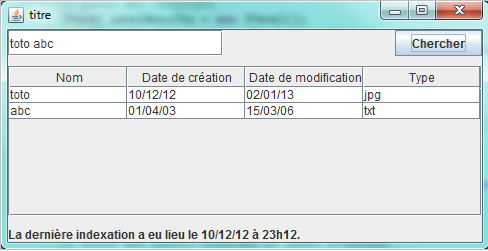
\includegraphics[scale=0.5]{figure1.png}
=======
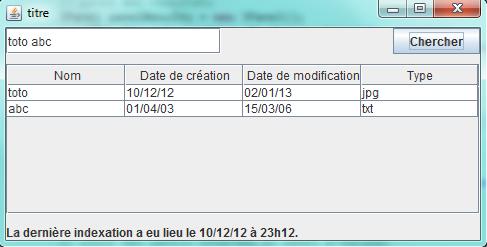
\includegraphics[scale=0.7]{rechercheSimple.png}
>>>>>>> ef841992d5df638244c7e73e4d6758b1363e056a
\caption{Recherche simple}
\end{figure}

Dans cet exemple, la recherche envoie tous les fichiers contenant les mots
"toto" ou "abc".

\subsection{Fonctionnalités du produit}
Lors de la première utilisation, iFind lance un démon ayant pour tâche d’indexer
un corpus ciblé. 
Ce démon va construire une base de données à l’aide de ces index. Un algorithme
est appliqué pour identifier dans le corpus (en utilisant l'index), les fichiers
qui correspondent le mieux aux mots contenus dans la requête, afin de présenter
les résultats des recherches par ordre de pertinence. Cette base de données va
jouer un rôle clé dans la phase de recherche de fichiers.
Ensuite, à chaque création ou modification de fichier appartenant au corpus, le
démon met à jour la base de données en fonction des modifications du fichier.

\subsection{User characteristics}

<<<<<<< HEAD
\section{Syntaxe MR}

\begin{center}
\begin{tabular}{| p{5cm} | p{8cm} |}
\hline
Minuscules/ majuscules & iFind ne tient pas compte de la casse des caractères.
Les requêtes 'ibm', 'Ibm' et 'IBM' renvoient le même résultat.\\
\hline
Lettres accentuées & \textbf{Important} \textit{electricite} et \textit{électricité}
ne donnent pas le même résultat, même si les différences sont souvent minimes.\\
\hline
<<<<<<< HEAD
Ordre des mots & \textbf{Important}: \textit{paris brest} donne un résultat 
différent de \textit{brest paris}. Une plus grande importance est donnée au premier 
mot choisi.\\
\hline
 Disjonction : Rechercher un mot ou  l'autre, requête -or requête
&
-or
Exemple : machin OR bidon. L'opérateur doit être saisi avec un tiret obligatoirement.\\
\hline
 Conjonction
 ET
& Opérateur par défaut
Exemple : 'moteur recherche' recherche les fichiers qui contiennent à la fois 'moteur' ET 'recherche'. 
Il est également possible d'utiliser le signe + pour demander une orthographe spécifique:
Exemple : +jéremie ne trouvera pas la forme "jeremie" (non accentuée)\\
\hline
 Exclure un mot
-e requête
&-e
Exemple : moteur –e automobile recherche les fichiers qui contiennent 'moteur' mais qui ne contiennent pas automobile.\\
=======
Ordre des mots & \textbf{Important}: \textit{paris brest } donne un résultat 
différent de \textit{brest paris}. Une plus grande importance est donnée au premier 
mot choisi.\\
\hline
Disjonction : Rechercher un mot ou  l'autre, requête -or requête
-or
Exemple : “machin OR bidon”. L'opérateur doit être saisi avec un tiret obligatoirement.
\hline
Conjonction
ET
Opérateur par défaut
Exemple : 'moteur recherche' recherche les fichiers qui contiennent à la fois 'moteur' ET 'recherche'. Il est également possible d'utiliser le signe + pour demander une orthographe spécifique :
Exemple : +jéremie ne trouvera pas la forme 'jeremie (non accentuée)
\hline
 Exclure un mot
-e requête
-e
Exemple : moteur –e automobile recherche les fichiers qui contiennent moteur mais qui ne contiennent pas automobile.
>>>>>>> ef841992d5df638244c7e73e4d6758b1363e056a
\hline
 Expressions & Non. Il n'est pas possible de faire des recherches de phrases exactes.\\
\hline
<<<<<<< HEAD
Troncature & Non. Il n'est pas possible de faire des recherches en utilisant la troncature sur iFind. 
le moteur recherche toujours exactement le mot demandé. 'mot' ne trouve pas 'mots' ni 'moteur'. L'astérique (*) ne peut pas être utilisé. 
iFind tient cependant parfois compte de la troncature, sans qu'il soit possible pour l'utilisateur de décider quand.\\
\hline
 Recherche sur le type de fichier
& -f
Exemple : exemples –f pdf. Plusieurs formats sont possibles.\\
\hline
 Recherche avancée & 
Advanced Search, Recherche avancée
Recherche sur le format de fichiers, sur la date de mise à jour, etc. Cependant, il n’y aura pas de syntaxe spécifique mais des boites de choix au niveau de l’interface graphique.\\
\hline
=======
Troncature
Non
Il n'est pas possible de faire des recherches en utilisant la troncature sur iFind. le moteur recherche toujours exactement le mot demandé. mot ne trouve pas mots ni moteur. L'astérique (*) ne peut pas être utilisé. iFind tient cependant parfois compte de la troncature, sans qu'il soit possible pour l'utilisateur de décider quand.
\hline
 Recherche sur le type   de fichier
-f
Exemple : exemples –f pdf. Plusieurs formats sont possibles.
\hline
 Recherche avancée
Advanced Search, Recherche avancée
Recherche sur le format de fichiers, sur la date de mise à jour, etc. Cependant, il n’y aura pas de syntaxe spécifique mais des boites de choix au niveau de l’interface graphique.

>>>>>>> ef841992d5df638244c7e73e4d6758b1363e056a

\end{tabular}
 
\end{center}



=======
\subsubsection{Syntaxe du moteur de recherche}

%\begin{tabular}{l{4cm} | c{4cm}}
\begin{tabular}{|p{4cm}|p{10cm}|}
%TODO SYNTAXE A DEFINIR
\hline
Minuscules/ majuscules & iFind ne tient pas compte de la casse des caractères.
Les requêtes 'ibm', 'Ibm' et 'IBM' renvoient le même résultat.\\
\hline
Lettres accentuées & \textbf{Important} \textit{electricite} et
\textit{électricité} ne donnent pas le même résultat, même si les différences
sont souvent minimes.\\
\hline
Ordre des mots & \textbf{Important}: \textit{paris brest } donne un résultat 
différent de \textit{brest paris}. Une plus grande importance est donnée au
premier 
mot choisi.\\
\hline
Disjonction : & Rechercher un mot ou  l'autre, \textit{requête -or requête}
Exemple : “machin OR bidon”. L'opérateur doit être saisi avec un tiret
obligatoirement.\\
\hline
Conjonction & Exemple : 'moteur recherche' recherche les
fichiers qui contiennent à la fois 'moteur' ET 'recherche'. Il est également
possible d'utiliser le signe + pour demander une orthographe spécifique :
Exemple : +jéremie ne trouvera pas la forme 'jeremie (non accentuée)\\
ET & \\
Opérateur par défaut & \\
\hline
Exclure un mot & Exemple : moteur –e automobile recherche les fichiers qui
contiennent moteur
mais qui ne contiennent pas automobile.\\
-e requête & \\
-e & \\
\hline
Expressions & Il n'est pas possible de faire des recherches de phrases
exactes.\\
Non & \\
\hline
Troncature & Il n'est pas possible de faire des recherches en utilisant la
troncature sur iFind. le moteur recherche toujours exactement le mot demandé.
mot ne trouve pas
mots ni moteur. L'astérique (*) ne peut pas être utilisé. iFind tient cependant
parfois compte de la troncature, sans qu'il soit possible pour l'utilisateur de
décider quand.\\
Non & \\
\hline
 Recherche sur le type   de fichier & Exemple : exemples –f pdf. Plusieurs
formats sont possibles.\\
 -f & \\
\hline
Recherche avancée & Recherche sur le format de fichiers, sur la date de mise à
jour, etc. Cependant,
il n’y aura pas de syntaxe spécifique mais des boites de choix au niveau de
l’interface graphique.\\
\hline
\end{tabular}
 
>>>>>>> ef841992d5df638244c7e73e4d6758b1363e056a
\subsubsection{Utilisation normale}
L'utilisateur entre une requête dans la barre de recherche.

\subsubsection{Utilisation avancée}
L'utilisateur peut également entrer une requête incluant des critères spéciaux
sur les fichiers à rechercher :
\begin{itemize}
 \item l'auteur
 \item la date de création
 \item la dernière date de modification
 \item le type
 \item la taille (pour les fichiers de type image)
 \item la durée (pour les fichiers de type musique ou vidéo)
\end{itemize}
Il est possible de paramétrer les fonctionnalités suivantes de l'indexation :
\begin{itemize}
 \item TODO
 \item TODO
\end{itemize}

% TODO INSERER ICI LA FIGURE
Figure 3

\subsection{Contraintes générales}
% TODO
Contraintes sur la recherche $\rightarrow$ si un fichier a été sauvegardé mais
pas quitté

\subsection{Dépendances}
Le logiciel sera utilisable sur une distribution GNU/Linux.
% TODO préciser les dépendances telles que “gcc” ou “java”

\end{document}
